
Duplicate content\textemdash{}memory pages and disk blocks\textemdash{}is a common
occurrence in virtualization-based hosting of applications, where
virtual machines (VMs) are instantiated from the same image 
template~\cite{effectiveness} or execute similar software environments. 
A study of content similarity amongst 525
virtual images from a production remote desktop environment~\cite{similarity}, 
reported that
30\% blocks were found to repeat at least twice and 12\% blocks were
found to repeat 5 times. A follow-up study~\cite{vdn}
reported median of pairwise similarity across
virtual machine images to be around 48\%.

Content similarity within a single virtual machine image is referred
as \textit{intra-VM}\index{Intra-VM} similarity, whereas 
across multiple images, it is
referred as \textit{inter-VM}\index{Inter-VM} similarity.
A study in \cite{intra-higherthan-inter} has reported that, in general,
intra-VM similarity is significant, with up to 90\% of total similarity 
observed among VM disk content being intra-VM.
The work in \cite{iodedup} studied the degree of 
content similarity\index{Content similarity}
in application workloads (web, mail and file system) hosted in 
individual virtual machines\index{Virtual machine},
and reported that the amount of unique content accessed is lesser
than the unique number of blocks accessed, implying that there are multiple 
blocks having identical content within each application workload.

\begin{figure}[t]
\centering
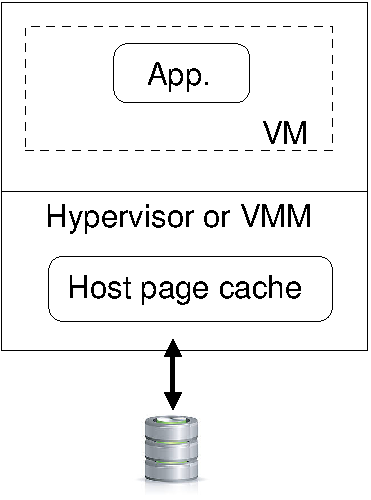
\includegraphics[scale=0.65]{confided-figures/main/system-under-considerat.pdf}
%\vspace{-0.15in}
\caption{Typical Virtualized System Under Consideration}
\label{fig:system-under-considerat}
%%\vspace{-0.2in}
\end{figure}

Consider the system illustrated in Fig.~\ref{fig:system-under-considerat}.
When an application or service (example, mail server or web server) is deployed 
within a VM instantiated on a host,
the virtual disk\index{Virtual disk} 
corresponding to the VM is present on the host's storage.
The storage may be a \textit{local} disk or a network-attached
\textit{remote} disk.
As discussed above, virtualized systems have inherent content similarity
among the data content that resides on disk, and this data is fetched 
from disk by corresponding applications. 
Disk access times are usually in the order of a few 
milliseconds\cite{google, data-domain}, whereas in comparison, 
host cache access timings are orders of magnitudes lower\cite{pagecache, satori}. 
Hence, improving caching
effectiveness can, in general, help improve storage access performance
and overall application performance.




%In the virtualized environment (refer Fig.\ref{fig:system-under-considerat}),
%both the VM and the host have
%their own page caches. A disk fetch by the host, on behalf of the VM, 
%results in the block being inserted in both the host cache and the VM cache. 
%This duplication of blocks across multiple
%caches in the hierarchy is referred as the \textit{cache inclusiveness}
%problem~\cite{my-cache-or-yours}. 
%Best practices~\cite{bestpractices} suggests to switch off the VM page-cache 
%so as to ensure that the entire cache space is used productively by the host
%itself. 
Due to the inherent similarity present in virtualized systems, the
effectiveness of the host's page-cache and overall application performance 
are impacted by two major factors:
(i)~\textit{duplicate I/O} problem~\cite{iodedup}, i.e.,
multiple blocks containing the same content being fetched from disk, and
(ii)~\textit{duplicate content} problem~\cite{satori,memorybuddies}, i.e.,
multiple blocks in cache have same content.
Both the duplicate I/O problem and duplicate content problem
can be addressed by actively maintaining metadata regarding the content 
similarity among blocks inserted into, and evicted from, the host page cache.
However, actively tracking the insertion and eviction of blocks in page cache
would require invasive changes in the host kernel. 


Harnessing content similarity 
to avoid duplicate disk I/O requests %that fetch the same content
is referred as I/O deduplication\index{I/O deduplication}.
To harness content similarity across different blocks,~\cite{iodedup} 
suggests the use of a 
\textit{content-based cache} which can be looked up by content also.
The proposed approach in \cite{iodedup} is to
maintain a \textit{content-based cache} and build 
metadata \index{Metadata}
regarding blocks inserted therein. 
A content-based cache\footnote{The terms 
\textit{content-cache} and \textit{content-based cache} are used 
interchangeably. Similarly for \textit{block-cache} and 
\textit{block-based cache}.}
can be referenced by content\index{Content-cache} 
(unlike a block-based\index{Block-cache} cache), and hence 
retains only a single copy of each content. 
It is used to intercept disk read
requests and deliver content directly, 
thus enabling I/O deduplication~\cite{iodedup}.
However, since only a fraction of total page cache space can be reserved
as an explicit content-cache, the remaining page cache still faces the
duplicate content problem (illustrated 
subsequently in Section~\ref{sec:thesis-iodedup}).

%commented because redundant.. else good para... 
% Work in \cite{iodedup} demonstrates that a 
% given limited size cache can be better utilized if used based on
% content, rather than blocks.
% However, by introducing a new content-cache, it introduces
% cache inclusiveness concerns among the two caches. Also, the
% split-cache design of reserving a part of existing block-cache as
% a content-cache implies that content-cache performance is
% achieved at the cost of precious block-cache space, as studied later
% in this chapter.

In this chapter, we present a read I/O redirection technique positioned within
the VM's virtual block device, such that both problems are 
addressed. If a block of content is present in the host's page-cache,
it need not get fetched from disk, i.e., I/O reduction is 
achieved. This, in turn, implies that multiple blocks with the same content 
are (almost) never stored into the host's page-cache, i.e., 
a content-deduplicated page-cache is achieved. 
Thus, our work is a deduplication-inspired technique for effective host
cache management.

The aim of this work is to achieve disk I/O reduction without actively 
tracking the state of the page-cache, as well as without maintaining any 
explicit content cache. 
We use a custom simulator to capture
the potential and benefits of the above approach.
The contributions of this work are, 
\begin{enumerate}
%In this paper, we present the
\item Simulation-based analysis of IODEDUP~\cite{iodedup}\index{IODEDUP} 
	system to show that it is 
	inefficient in terms of achieving the goal of I/O deduplication.
  \item Design and implementation of the DRIVE\index{DRIVE} 
	module that tackles both the
	duplicate content problem and the duplicate I/O problem
\item Extensive trace-based evaluation of DRIVE with prototype
	implementation within a custom simulator.
\end{enumerate}

%\footnote{The terms \textit{block-cache} and 
%\textit{block-based cache} are used
%interchangeably. Similarly for \textit{content-cache} and 
%\textit{content-based cache}.}

%Building an integrated block-based and 
%content-based cache would help utilize cache space more 
%effectively, but 
%such integration would make the system design highly complex
%with invasive changes required in existing kernel.
%Hence, we propose a request redirection
%technique positioned above the block-cache, such that it implicitly 
%manipulates cache usage, without being invasive. 
%We build DRIVE, a storage access optimization that
%identifies content similarity at block level, and 
%redirects requests 
%to better
%manage the existing block-based cache as a content-based cache.

%The contributions in this work are the following:
%(i)~Demonstrate that existing work addresses only one of the problems
%of duplicate I/O and duplicate content at a time, and hence falls short
%of exploiting the host's page-cache space to its maximum.
%%introduces additional cache inclusiveness
%%problem by using an explicit content-based cache.
%%Highlighting the problem with split-cache based design, hence
%%motivating the need for a content-deduplicated cache,
%%(ii)~Design and implementation of DRIVE system which
%%performs read I/O request redirection to achieve integrated cache effect, 
%%and
%(ii)~Design and implementation of DRIVE system that tackles both the
%duplicate content problem and duplicate I/O problem in one stroke,
%and
%(iii)~Extensive trace-based evaluation of DRIVE with prototype 
%implementation within a simulation module.
%%split-cache approach as well as the Vanilla system.
